% Created 2022-11-24 jue 13:09
% Intended LaTeX compiler: pdflatex
\documentclass[10pt]{article}
\usepackage[utf8]{inputenc}
\usepackage[T1]{fontenc}
\usepackage{graphicx}
\usepackage{grffile}
\usepackage{longtable}
\usepackage{wrapfig}
\usepackage{rotating}
\usepackage[normalem]{ulem}
\usepackage{amsmath}
\usepackage{textcomp}
\usepackage{amssymb}
\usepackage{capt-of}
\usepackage{hyperref}
\usepackage[spanish]{babel}
\usepackage{graphicx,geometry}
\geometry{ a4paper, left=1in, right=1in, top=1in, bottom=1in }
\renewcommand\familydefault{\sfdefault}
\usepackage{sectsty}
\sectionfont{\normalfont\Large }
\subsectionfont{\normalfont\normalsize}
\usepackage{tabularx}
\usepackage{listings}
\lstdefinestyle{mystyle}{
numbers=left,
showspaces=false,
frame=single,
showspaces=false,
showstringspaces=false,
showtabs=false,
numberstyle=\tiny,
aboveskip=\parskip,
basicstyle=\ttfamily\footnotesize
}
\lstset{
style=mystyle,
literate={á}{{\'a}}1
{é}{{\'e}}1
{í}{{\'{\i}}}1
{ó}{{\'o}}1
{ú}{{\'u}}1
{Á}{{\'A}}1
{É}{{\'E}}1
{Í}{{\'I}}1
{Ó}{{\'O}}1
{Ú}{{\'U}}1
{ü}{{\"u}}1
{Ü}{{\"U}}1
{ñ}{{\~n}}1
{Ñ}{{\~N}}1
{¿}{{?``}}1
{¡}{{!``}}1
}
\makeatletter
\usepackage{fancyhdr}
\pagestyle{fancy}
\usepackage{mdframed}
\BeforeBeginEnvironment{minted}{\begin{mdframed}}
\AfterEndEnvironment{minted}{\end{mdframed}}
\author{Luis Eduardo Galindo Amaya (1274895)}
\date{23-11-2022}
\title{Prueba de normalidad analítica}
\hypersetup{
 pdfauthor={Luis Eduardo Galindo Amaya (1274895)},
 pdftitle={Prueba de normalidad analítica},
 pdfkeywords={},
 pdfsubject={},
 pdfcreator={Emacs 26.3 (Org mode 9.1.9)}, 
 pdflang={Spanish}}
\begin{document}


\newcommand{\docente}{Olivia Mendoza Duarte}
\newcommand{\asignatura}{Estadística Avanzada}
\newcommand{\semestre}{2022-2}

\newcommand{\miportada}[1]{
	\begin{titlepage}
		\vspace*{0.75in}
		\begin{flushleft}
			\sffamily
			\large #1       \\
			\Huge
            \@title         \\
			\hrulefill
			\vspace{0.25in} \\
			\Large \@author \\
			%% \vspace*{\fill}
            %% 
\includegraphics[width=\textwidth]{../includes/filler.png} \\
			\vspace*{\fill}
			\large
			\begin{tabular}{|l|l|}
              \hline
			  Asignatura & \asignatura \\
			  Docente    & \docente    \\
			  Fecha      & \@date      \\
              \hline
			\end{tabular}
		\end{flushleft}
	\end{titlepage}
}

\miportada{ Práctica 11 }

\fancyhf{}
\lhead{ \asignatura }
\rhead{ \semestre }
\rfoot{Página \thepage}

\setlength\parindent{0pt}   % eliminar el intentado
\setlength{\parskip}{1.2em}

\maketitle
\end{center}

\section*{Información del dataset\footnote{\url{https://archive-beta.ics.uci.edu/ml/datasets/iris}}}
\label{sec:org072801f}
This is one of the best known datasets in statistics and machine learning.  Fisher's paper is a classic in the field and is frequently used for tutorial and teaching purposes. The data set contains 3 classes of 50 instances each, where each class refers to a type of iris plant.  One class is linearly separable from the other 2; the latter are not linearly separable from each other.

Predicted attribute: class of iris plant.

\begin{enumerate}
\item sepal length
\item sepal width
\item petal length
\item petal width
\item class
\end{enumerate}

\section*{Desarollo de la práctica}
\label{sec:org6b665f9}
\subsection*{Distribusion normal (sepal width)}
\label{sec:org0e94c68}
\subsubsection*{Observacion previa}
\label{sec:org81621c8}
Se puede notar como el ancho del sépalo se distribuye de manera normal, el tamaño del sépalo tiende a ser de un tamaño especifico y no tanto del tamaño de los pétalos 

\subsubsection*{Resultados}
\label{sec:orgece9e67}
Efectivamente los valores coinciden en una distribucion normal \(RQ = 0.9925113\).

\begin{figure}[htbp]
\centering
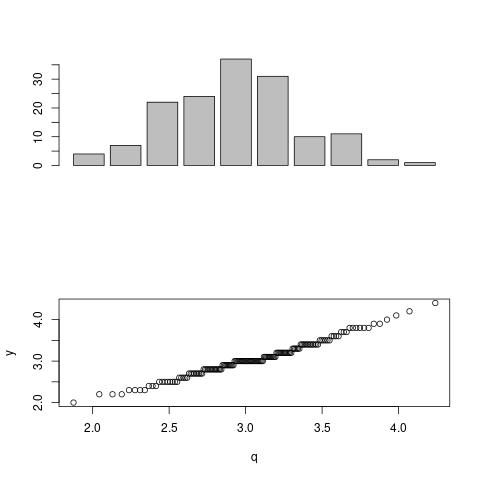
\includegraphics[width=7cm]{img/i1.jpeg}
\caption{columna ''sepal width''}
\end{figure}



\subsection*{Distribucion no normal (sepal length)}
\label{sec:orgee5ee91}
\subsubsection*{Observacion previa}
\label{sec:org4ab1fe1}
El largo del sépalo se distribuye de manera serrada sobre los datos, no parece haber un patrón en la gráfica

\subsubsection*{Resultados}
\label{sec:org67de33c}
Aunque de a primera vista no es muy claro los datos de esta columna tambien cumplen la prueba de normalidad \(rQ = 0.9891878\).

\begin{figure}[htbp]
\centering
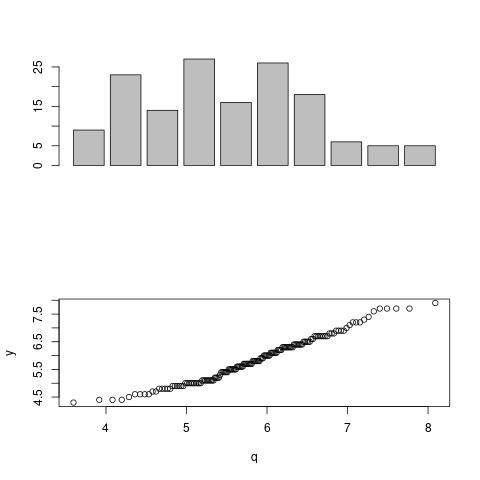
\includegraphics[width=7cm]{img/i2.jpeg}
\caption{columna ''sepal length'' del dataset bezdekIris}
\end{figure}

\subsection*{Distribucion no normal (petal length)}
\label{sec:org14834fc}
\subsubsection*{Observacion previa}
\label{sec:org31b8f16}
Por otro lado el largo de los pétalos es muy interesante, en la parte derecha parece haber una distribución normal pero tiene unos sectores que sobresalen a la izquierda.

\subsubsection*{Resultados}
\label{sec:org555b294}
Esta no es una distribución normal, la gráfica sale completamente dividida \(rQ = 0.9378633\)

\begin{figure}[htbp]
\centering
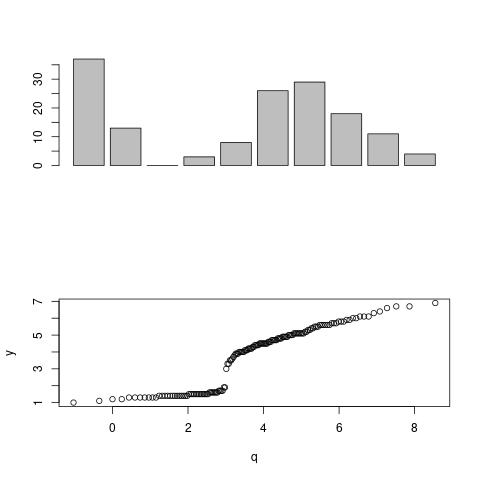
\includegraphics[width=7cm]{img/i3.jpeg}
\caption{columna ''petal length'' del dataset bezdekIris}
\end{figure}

\section*{Conclusiones}
\label{sec:org7f4d2f7}
Usar métodos que solo dependen de la observación es bastante peligroso, ya que no podemos determinar con total precisión si nuestras gráficas coinciden o no y que un simple cambio en el numero de clases puede hacer que la gráfica sea completamente diferente, el método analítico nos permite tener mucha precisión para determinar si nuestros casos coinciden

\section*{Código}
\label{sec:orgedd47ae}
\lstinputlisting{./pruebaDeNormalidad.R}
\end{document}
